
\section{Headtracking}

Ziel des Headtrackings ist es, die Kopforientierung des Fahrers --auch bei bewegtem Fahrzeug-- sowohl relativ zum Fahrzeug als auch in Weltkoordinaten anzugeben.

Dazu wird die Inertialsensorik der \ac{AR}-Brille, bestehend aus zwei Gyroskopen, Beschleunigungssensor und Magnetometer, ausgewertet (Abs. \ref{headtracking_imu_subsec}).
Diese Daten werden mit einem geeigneten Filter-Algorithmus fusioniert (Abs. \ref{headtracking_fusion_subsec}).
Die Kompensation der Eigenbewegung des Fahrzeugs wird in Abs. \ref{headtracking_marker_subsec} behandelt.


\subsection{Inertialsensoren}
\label{headtracking_imu_subsec}


\subsubsection{Gyroskop}

Funktionsweise
Tiefpassfilter
Bias-Korrektur
HBW \& LBW Fusion
Wertebereiche, wie alte Präsentation
Integration
Eigenschaften (schnell, aber Drift durch Integration)


\subsubsection{Beschleunigungssensor}

Funktionsweise
für Roll und Pitch
Tiefpassfilter
Umrechnung auf m/s$^2$
Berechnung von Roll und Pitch direkt aus Werten
Problem: ungenügendes Yaw


\subsubsection{Magnetometer}

Das Magnetometer wird im Rahmen des Praktikums zur Stützung des Yaw-Winkels (Drehung um die Z-Achse des Brillenkoordinatensystem) genutzt.\\
Das verbaute Magnetometer misst in drei Achsen nach dem Funktionsprinzip der Wheatstonesche Messbrücke \cite{renaudin2010complete} das Erdmagnetfeld.
Dieses Messverfahren führt zum einen zu einer kleinen und kostengünstigen Bauweise.
Zum anderen entstehen aber Messungenauigkeiten, die im Rahmen der Sensorkalibrierung beachtet und ausgeglichen werden müssen.
Gemessen werden die Magnetfeldlinien der Erde.
Diese sind abhängig von der aktuellen Position auf der Erdoberfläche\footnote{Tatsächlich verändert sich das Erdmagnetfeld auch über die Zeit hinweg.
Diese Änderung kann aber im Rahmen des Praktikums vernachlässigt werden, da es sich um eine sehr kleine Änderung handelt (z. Bsp. für den Praktikumsort Karlsruhe ca. $1^\circ 46$'~$7.8$ arcmin/Jahr im Deklinationswinkel).}.

Der gemessene 3D-Magnetfeldvektor ist somit zunächst unkalibriert und laut der Spezifikation im Datenblatt \todo{cite} einheitenlos.
Daher ist zuerst eine Kalibrierung der gemessenen Werte notwendig um sie weiterverarbeiten zu können.
Im Gegensatz zu den bisher vorgestellten Sensoren wird die Kalibrierung des Magnetometers durch Bewegung durchgeführt.
Ziel ist es, die Wertebereiche in allen drei Achsen zu erfassen.
Dafür wird die Brille in allen Achsen um mindestens $360^\circ$ gedreht, um die minimalen und maximalen Werte zu registrieren. \ldots Wie in Abbildung \ref{fig:mag_world}\ldots



Funktionsweise

\begin{figure}
   \centering
   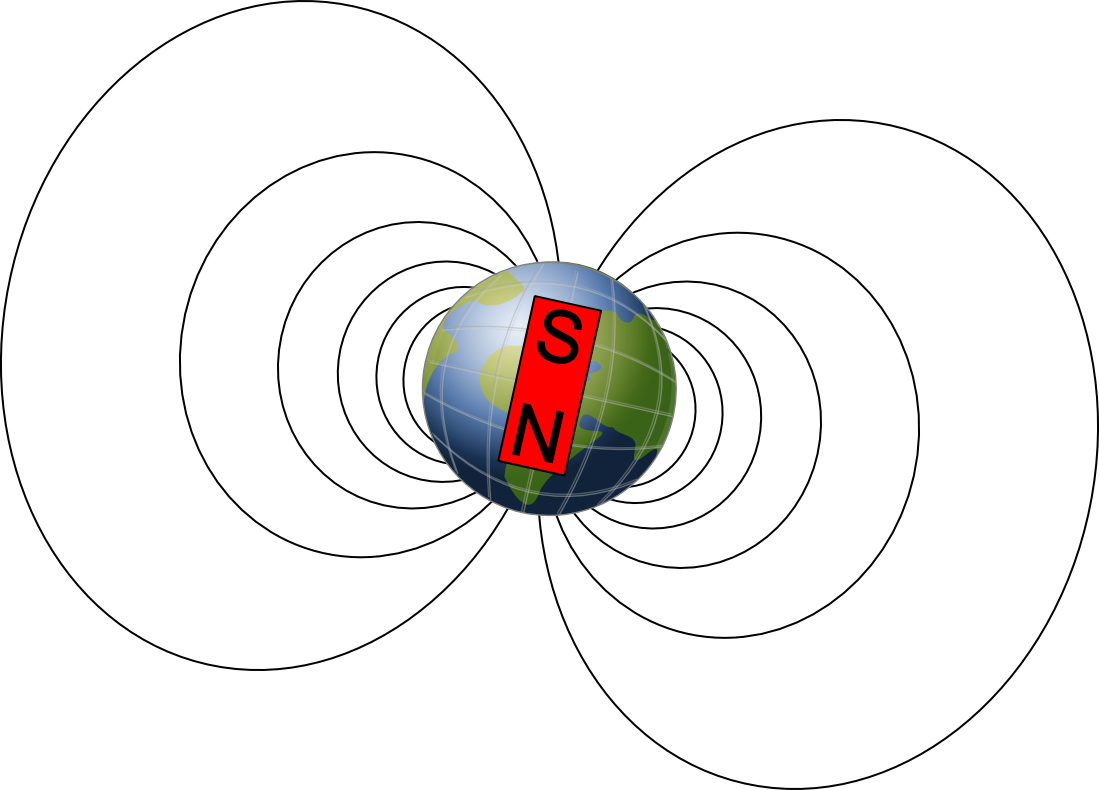
\includegraphics[width=0.3\textwidth]{earth-magnetic-field}
   \caption[mag_world]{Schematische Darstellung des Erdmagnetfelds.}
   \label{fig:mag_world}
\end{figure}
\todo{cite Erdmagnetfeld}

Tiefpassfilter
Magnetometer-Bias-Korrektur (durch Min/Max-Werte), Normierung auf [-1,1]
Magnetometer-Kreisplots vor/nach Kalibrierung, Magnetometer-Fehler in Kreisplots
Transformation auf XY Ebene (Algorithmus Ralf)


